%% Generated by Sphinx.
\def\sphinxdocclass{report}
\documentclass[letterpaper,12pt,english]{sphinxmanual}
\ifdefined\pdfpxdimen
   \let\sphinxpxdimen\pdfpxdimen\else\newdimen\sphinxpxdimen
\fi \sphinxpxdimen=.75bp\relax
\ifdefined\pdfimageresolution
    \pdfimageresolution= \numexpr \dimexpr1in\relax/\sphinxpxdimen\relax
\fi
%% let collapsable pdf bookmarks panel have high depth per default
\PassOptionsToPackage{bookmarksdepth=5}{hyperref}

\usepackage{graphicx}
\usepackage{babel}

\PassOptionsToPackage{warn}{textcomp}
\usepackage[utf8]{inputenc}
\ifdefined\DeclareUnicodeCharacter
% support both utf8 and utf8x syntaxes
  \ifdefined\DeclareUnicodeCharacterAsOptional
    \def\sphinxDUC#1{\DeclareUnicodeCharacter{"#1}}
  \else
    \let\sphinxDUC\DeclareUnicodeCharacter
  \fi
  \sphinxDUC{00A0}{\nobreakspace}
  \sphinxDUC{2500}{\sphinxunichar{2500}}
  \sphinxDUC{2502}{\sphinxunichar{2502}}
  \sphinxDUC{2514}{\sphinxunichar{2514}}
  \sphinxDUC{251C}{\sphinxunichar{251C}}
  \sphinxDUC{2572}{\textbackslash}
\fi
\usepackage{cmap}
\usepackage[T1]{fontenc}
\usepackage{amsmath,amssymb,amstext}
\usepackage{babel}
\usepackage{booktabs}
\usepackage{multirow}
\usepackage{setspace}
\usepackage{graphicx}
\usepackage{subcaption}
\usepackage[flushleft]{threeparttable}
\usepackage{lscape}
\usepackage{rotating}
\usepackage{array}
\usepackage{setspace}
\usepackage{caption}
%\usepackage{apalike}
\usepackage[export]{adjustbox}
\usepackage{array}
\usepackage{amsmath}
\usepackage{breqn}
\usepackage{enumitem}
\usepackage[table, x11names]{xcolor}

\usepackage{tgtermes}
\usepackage{tgheros}
\renewcommand{\ttdefault}{txtt}

\renewcommand{\baselinestretch}{1.15} 

\newcommand{\tabitem}{\hspace*{0.5cm}\llap{\textbullet}~~}
\newcommand{\subtabitem}{\hspace*{1cm}\llap{--}~~}

\usepackage[Bjarne]{fncychap}
\usepackage{sphinx}

\usepackage{chngcntr}
\counterwithout{figure}{chapter}
\counterwithout{table}{chapter}

%\fvset{fontsize=auto}
\usepackage{geometry}


% Include hyperref last.
\usepackage{hyperref}
% Fix anchor placement for figures with captions.
\usepackage{hypcap}% it must be loaded after hyperref.
% Set up styles of URL: it should be placed after hyperref.
\urlstyle{same}

\addto\captionsenglish{\renewcommand{\contentsname}{Table of Contents}}

\usepackage{sphinxmessages}
\setcounter{tocdepth}{1}


\title{DREAMIN'SG Integrated Power-Water-Transportation Simulation}
\date{\today}
\release{User Manual v1.0}
\author{Srijith Balakrishnan\\ Beatrice Cassottana\\ Felix Kottmann}
\newcommand{\sphinxlogo}{\vbox{}}
\renewcommand{\releasename}{}
\makeindex
\begin{document}

\pagestyle{empty}
\sphinxmaketitle
\pagestyle{plain}
\sphinxtableofcontents
\pagestyle{normal}

\chapter{Introduction}
This package is developed as part of the Disaster REsilience Assessment, Modelling, and INnovation Singapore (DREAMIN’SG) project at the Future Resilient Systems of the Singapore ETH Centre. The DREAMIN'SG project is funded by the National Research Foundation, Singapore under the Intra-CREATE grant program. In the wake of increasing threats posed by climate change on urban infrastructure \cite{Nissen2017}, this project aims at studying the effects of policy interventions and network characteristics on the resilience of urban infrastructure networks. Given the critical nature of the above infrastructure systems, their interdependencies need to be considered in pre- and post-disaster resilience actions. 


In specific, the DREAMIN'SG project envisages to build a methodology to assess and predict the resilience of urban infrastructure systems and propose new pathways to develop innovative technologies and services for its improvement. The urban infrastructure system is modeled as an interdependent power-, water-, and transportation network that interact with each other before, during and after a disaster. The researchers are developing an integrated simulation model to study the performance of the interdependent infrastructure network under various disruption and recovery scenarios. Based on the simulation-generated datasets, machine learning algorithms would be implemented to understand the causal relationship between topological and policy-related interventions and disaster risks. Building on the understanding of success features that make an urban system resilient, Design Science approaches will be used to develop new solutions that mitigate the consequences of disruptions and accommodate constraints in the analysed case studies. The results of the research will support local governments and system managers to improve infrastructure resilience against weather-related disruptions. The methodology adopted in the study is presented in Fig.~\ref{fig:method}.

The steps of the project are summarized as follows:
\begin{enumerate}[noitemsep]
	\item Multiple scenarios are generated by considering different disruptions, network models, technological constraints and system configurations. 
	\item A simulation model is created for the interdependent power grid, water distribution system, and road transportation system. 
	\item Resilience is assessed based on the simulated performance of the three systems. 
	\item An interpretable machine learning algorithm is implemented to analyze the scenarios and extract information related to key system features that influence resilience.
	\item The identified system features inform the design of new services, technologies, and products that are able to simultaneously enhance resilience and accommodate the technological constraints. 
\end{enumerate}

\begin{figure}[htbp]
	\centering
	\noindent\sphinxincludegraphics[width = \textwidth]{{methodology}.PNG}
	\caption{Methodological framework of DREAMIN’SG project}\label{fig:method}
\end{figure}


For further information and updates on the project, please visit the
DREAMIN'SG project webpage \footnote{Disaster REsilience Assessment, Modelling, and INnovation Singapore  ~\sphinxhref{https://frs.ethz.ch/research/projects/dreamin\_sg.html}{https://frs.ethz.ch/research/projects/dreamin\_sg.html}}. In the rest of the report, the details of the interdependent infrastructure simulation platform, including its modeling, installation, and usage are discussed.


\chapter{Integrated Simulation Platform}
\label{\detokenize{index:integrated-simulation-platform}}
\sphinxAtStartPar
The integrated simulation model has been developed as a Python\sphinxhyphen{}based package consisting of modules for simulation of system\sphinxhyphen{} and network\sphinxhyphen{}level
cascading effects resulting from component failures. The overall structure of the integrated simulation platform is illustrated in Fig.~\ref{fig:framework}.

\begin{figure}[htbp]
\centering
\capstart
\noindent\sphinxincludegraphics[width = \textwidth]{{structure}.PNG}
\caption{DREAMIN’SG integrated simulation platform structure}\label{fig:framework}\end{figure}

\sphinxAtStartPar
The model is capable of initializing disaster scenarios in interdependent power, water and transportation networks and evaluating resilience strategies by generating operational performance curves (Fig.~\ref{fig:perf_curves}). The resilience strategies that can be tested include pre-disaster interventions, such as system redundancy enhancements and post-disaster recovery optimization.

\begin{figure}[htbp]
\centering
\capstart

\noindent\sphinxincludegraphics[width=\textwidth]{perf_curves.PNG}
\caption{Implementation of the simulation platform to generate performance curves}\label{fig:perf_curves}\end{figure}

\sphinxAtStartPar
The model is developed by integrating existing flow\sphinxhyphen{}based water, power and transportation network models. The whole model can be divided into three broad modules, namely, the integrated infrastructure network module, network recovery module, and the recovery optimization module.


\section{Integrated infrastructure network}
\label{\detokenize{index:integrated-infrastructure-network}}
\sphinxAtStartPar
This module houses the three infrastructure network models which are used to simulate power-, water-, and transportation networks independently.  These are developed using existing Python\sphinxhyphen{}based packages. In order to model the power network, \texttt{pandapower} was used \cite{Thurner2018}. The water distribution network is modeled using \texttt{wntr} package \cite{Klise2020}. The traffic network is modeled using static traffic assignment method \cite{Boyles2020}. The details of the packages are presented in Table~\ref{tab:infra_packages}

The module also consists of an interdependency sub-module which serves as an interface between infrastructure network pairs. Currently the following dependencies are considered in the interdependent simulation platform.

\begin{enumerate}[noitemsep]
\item Power-water dependencies include dependency of water pumps on electric motors and generators on reservoirs.
\item Dependencies also exist between traffic network and the other two infrastructure models, as the former provides access to the latter. The disruptions to transportation infrastructure components are their recovery are key considerations that affect the restoration and recovery of all other infrastructure networks. The module also stores the details of the states of all network components, including their operational status after a disaster.

\end{enumerate}

\begin{table}[htbp]
	\caption{Infrastructure packages using in the simulation model}
	\begin{tabular}{p{0.15\textwidth}p{0.2\textwidth}p{0.6\textwidth}}
		\cellcolor[HTML]{C0C0C0}Infrastructure & \cellcolor[HTML]{C0C0C0}Package & \cellcolor[HTML]{C0C0C0}Capabilities\\ 
		Power & \texttt{pandapower} & 
		\begin{minipage}[t]{0.6\textwidth}
			\begin{itemize}[leftmargin=6pt,noitemsep,nolistsep,after=\strut]
				\item Capable of generating power networks with standard components such as lines, buses, and transformers based on design data.
				\item Capable of performing power-flow analysis.
			\end{itemize}
		\end{minipage} \\
		\cellcolor[HTML]{EFEFEF}Water & \cellcolor[HTML]{EFEFEF}\texttt{wntr} & \cellcolor[HTML]{EFEFEF}\begin{minipage}[t]{0.6\textwidth}
			\begin{itemize}[leftmargin=6pt,noitemsep,nolistsep,after=\strut]
				\item Capable of generating water networks with standard components such as pipes, tanks, and nodes based on design data.
				\item Capable of performing pressure dependent demand or demand-driven hydraulic simulations.
			\end{itemize}
		\end{minipage} \\
		Transportation & static traffic assignment package & 
		\begin{minipage}[t]{0.6\textwidth}
			\begin{itemize}[leftmargin=6pt,noitemsep,nolistsep,after=\strut]
				\item Capable of implementing static traffic assignment and computing travel times between origin-destination pairs.
			\end{itemize}
		\end{minipage} \\
		\end{tabular}
	\label{tab:infra_packages}
	\end{table}

\section{Network recovery}
\label{\detokenize{index:network-recovery}}
\sphinxAtStartPar
The recovery module consists of functions to develop an event table to schedule disruptive events and restoration actions after a disaster
is initiated in the model. The simulation platform uses this table as a reference to modify the operational status of network components
during a simulation, so that the consequences of disaster events and repair actions are reflected while simulating network performance. The
recovery module also stores the details such as the number of repair crew for every infrastructure network, their initial locations, etc.


\section{Recovery optimization}
\label{\detokenize{index:recovery-optimization}}
\sphinxAtStartPar
This module determines the order in which the repair actions are carried out. Currently, the approach of the optimization module leverages
on the methodology of Model Predictive Control (MPC) \cite{Camacho2007}. In this approach, first, out of \sphinxstyleemphasis{N} repair steps, the solution considering only \sphinxstyleemphasis{k} steps,
called the prediction horizon, is computed. Next, the first step of the obtained solution is applied to the system and then the process is
being repeated for the remaining \sphinxstyleemphasis{N\sphinxhyphen{}1} components until all components have been scheduled for repair. In the context of the integrated infrastructure simulation, the optimizer module evaluates repair sequences of the length of the prediction horizon for each infrastructure (assuming that each of the infrastructure has a separate recovery crew) based on a resilience metric. In the model, the integral loss of service (ILOS) is used as the
resilience metric. The ILOS is calculated as follows:

\begin{equation}
\begin{split}ILOS = w_{P}\sum_{k}\Delta Power\times dt_{P}(k)+w_{W}\sum_{k}\Delta Water\times dt_{w}(k)+w_{T}\sum_{k}\Delta Transport\times dt_{T}(k)\end{split}
\end{equation}

\sphinxAtStartPar
where, \(\Delta Power\), \(\Delta Water\) and \(\Delta Transport\) are the respective demands not served, \(dt_{P}(k)\), \(dt_{W}(k)\) and \(dt_{T}(k)\) the repair\sphinxhyphen{}time specific time steps between the repair actions and \(w_{P}\), \(w_{W}\), \(w_{T}\) the weights. The optimal repair sequence is found by minimizing the ILOS. At this stage, the optimal repair action in each prediction horizon is computed using a brute\sphinxhyphen{}force approach where the ILOS is evaluated for each of the repair sequences.

\section{Work in progress}
Currently, the network data, interdependency data and infrastructure disruption data are to be manually fed into the model to run the network simulations.
However, efforts are being made to include separate modules for network generation and hazard initiation in the simulation platform, to enhance the scope of the model.
The following improvements will also be made to the model:
\begin{enumerate}[noitemsep]
\item Realistic policies for network recovery.
\item Additional interdependencies.
\item More efficient repair optimization algorithms
\end{enumerate}

\chapter{Model Data requirements}

Currently, network generation and hazard generation are not automated in the integrated simulation model. Therefore, in order to use the model, three types of data are to be manually fed into the model, namely the water, power and transportation networks, interdependency data, and infrastructure disruption data. There datasets need to be in specific formats which are compatible with the model. In this chapter, the details such as file formats and information to be included in the input files are discussed in detail. 

\section{Infrastructure networks}
The infrastructure network data must be compatible with the respective infrastructure model packages enlisted in Table~\ref{tab:infra_packages}. In addition, disruptions to certain components belonging to the infrastructure systems are not supported as of now. The individual networks must be constructed taking into the above aspects into consideration.

\subsection{Water distribution system}
Since the integrated simulation model handles the water distribution network models using {\tt wntr} package, the input file must be in {\tt .inp} format. Some examples of water network files can be found in {\tt wntr} Github repository\footnote{\href{https://github.com/USEPA/WNTR/tree/main/examples/networks}{https://github.com/USEPA/WNTR/tree/main/examples/networks}}. The water network can be either built using EPANET or {\tt wntr} package. Currently, the water network simulation is performed using {\tt WNTRSimulator} in the {\tt wntr} package. Therefore, there are certain exceptions which must be considered while generating the water network file. These exceptions can be found in {\tt wntr}'s software framework and limitations\footnote{Software framework and limitations. \href{https://wntr.readthedocs.io/en/latest/framework.html\#discrepancies}{{https://wntr.readthedocs.io/en/latest/framework.html\#discrepancies}}} page.

In addition, the integrated simulation model identifies the component details such as infrastructure type, component type, etc. using the component names. The name of the components must follow the nomenclature. The details of nomenclature and whether a component can be failed in the model is presented in Table~\ref{tab:water_compons}. For example, a water pump can be named as {\tt W\_WP1}. Integers must be followed by the prefix to name components belonging to same category.

\begin{table}[h]
	\centering
	\caption{Nomenclature and disruption functionality of supported water system components}
	\begin{tabular}{lll}
		\rowcolor[HTML]{C0C0C0} 
		Prefix & Component name & Disruption supported \\
		W\_WP  & Pump           & Yes                 \\
		\rowcolor[HTML]{EFEFEF} 
		W\_R   & Reservoir      & No                  \\
		W\_P   & Pipe           & Yes                 \\
		\rowcolor[HTML]{EFEFEF} 
		W\_J   & Junction       & No                  \\
		T      & Tank           & Yes                
	\end{tabular}
\label{tab:water_compons}
\end{table}

\subsection{Power system}
The power system is modeled using {\tt pandapower} package, and therefore the network file must be in {\tt *.json} format. Several tutorials for generating power system networks using {\tt pandapower} are available in the package's tutorial page\footnote{\href{https://github.com/e2nIEE/pandapower/tree/develop/tutorials}{https://github.com/e2nIEE/pandapower/tree/develop/tutorials}}. Similar to water network components, naming of power system components must also follow the stipulated nomenclature presented in Table~\ref{tab:power_compons}. Currently, power networks are modeled as three-phase systems. Therefore, single-phase components in {\tt pandapower} are not supported. Integers must be followed by the prefix to name components belonging to same category.

\begin{table}[h]
	\centering
	\caption{Nomenclature and disruption functionality of supported power system components}
	\begin{tabular}{lll}
		\rowcolor[HTML]{C0C0C0} 
		Prefix & Component name              & Disruption supported \\
		P\_B      & Bus                         & Yes                 \\
		\rowcolor[HTML]{EFEFEF} 
		P\_LOA    & Asymmetric load             & Yes                 \\
		P\_LOMP   & Motor as load               & Yes                 \\
		\rowcolor[HTML]{EFEFEF} 
		P\_AL     & Asymmetric load             & Yes                 \\
		P\_AS     & Asymmetric static generator & No                  \\
		\rowcolor[HTML]{EFEFEF} 
		P\_SW     & Switch                      & Yes                 \\
		P\_EG     & External Grid               & Yes                 \\
		\rowcolor[HTML]{EFEFEF} 
		P\_L      & Line                        & Yes                 \\
		P\_TF     & Transformer                 & Yes                
	\end{tabular}
\label{tab:power_compons}
\end{table}

\subsection{Transportation system}
The transportation system is simulated using the static traffic assignment model developed by Prof. Stephen Boyles of Department of Civil, Architectural and Environmental Engineering, The University of Texas at Austin. The transportation network data must be in the TNTP data format. More details on the format and example networks can be found in Ben Stabler's Github page\footnote{\href{https://github.com/bstabler/TransportationNetworks}{https://github.com/bstabler/TransportationNetworks}}. The naming of the transportation network components must follow the nomenclature presented in Table~\ref{tab:transpo_compons}. Integers must be followed by the prefix to name components belonging to same category.

\begin{table}[h]
	\centering
	\caption{Nomenclature and disruption functionality of supported transportation system components}
	\begin{tabular}{lll}
		\rowcolor[HTML]{C0C0C0} 
		Prefix & Component name & Disruption supported \\
		T\_J   & Junction       & No                   \\
		\rowcolor[HTML]{EFEFEF} 
		T\_L   & Link           & Yes                 
	\end{tabular}
\label{tab:transpo_compons}
\end{table}

\section{Infrastructure dependencies}
Data related to water-power dependencies\footnote{The dependencies of power and water networks on transportation network are identified internally by the model and therefore that information need not be provided in the dependency data file.} between infrastructure components must be provided separately in a {\tt .csv} file. The file must contain {\tt water\_id} and {\tt power\_id} fields which represent the water- and power component names (Table~\ref{tab:interdependencies}). The model will determine the type of the water- and power components and construct the dependencies accordingly. 

\begin{table}[h]
	\centering
	\caption{Format of dependency data file}
	\begin{tabular}{ll}
		\rowcolor[HTML]{C0C0C0} 
		water\_id & power\_id name \\
		W\_WP9   & P\_MP1       \\
		\rowcolor[HTML]{EFEFEF} 
		W\_R9   & P\_G3     
	\end{tabular}
	\label{tab:interdependencies}
\end{table}

\section{Infrastructure disruption data}
The third data input is related to disrupted components. Similar to the dependency input file, the disruption data also needs to be provided in {\tt *.csv} format. The file should have three fields, namely {\tt time_stamp} (time of disruption in seconds), {\tt components} (name of the component that is included in any of the three networks), and {\tt fail_perc} (percentage of damage). An example for the dependency data is presented in Table~\ref{tab:disruptive_events}.

\begin{table}[h]
	\centering
	\caption{Disruptive event table generated from dependencies input file}
	\begin{tabular}{crlr}
		\multicolumn{1}{l}{} &
		\multicolumn{1}{l}{\cellcolor[HTML]{C0C0C0}time\_stamp} &
		\cellcolor[HTML]{C0C0C0}components &
		\multicolumn{1}{l}{\cellcolor[HTML]{C0C0C0}fail\_perc} \\
		0 &
		\cellcolor[HTML]{FFFFFF}15000 &
		\cellcolor[HTML]{FFFFFF}P\_MP1 &
		\cellcolor[HTML]{FFFFFF}75 \\
		1 &
		\cellcolor[HTML]{EFEFEF}6000 &
		\cellcolor[HTML]{EFEFEF}T\_L2 &
		\cellcolor[HTML]{EFEFEF}50
	\end{tabular}
	\label{tab:disruptive_events}
\end{table}

While the percentage of damage of component is not used in the current model, this may be incorporated in the model to find the repair duration estimate in the future versions.


\chapter{Installation}
\label{\detokenize{index:installation}}

\section{Stable release}
\label{\detokenize{index:stable-release}}
\sphinxAtStartPar
To install dreaminsg\sphinxhyphen{}integrated\sphinxhyphen{}model, run this command in your terminal\footnote{Currently, the package is not uploaded to PyPI repository. However, it will be done in the near future.}:

\begin{sphinxVerbatim}[commandchars=\\\{\}]
\PYG{g+gp}{\PYGZdl{} }pip install dreaminsg\PYGZus{}integrated\PYGZus{}model
\end{sphinxVerbatim}

\sphinxAtStartPar
This is the preferred method to install dreaminsg\sphinxhyphen{}integrated\sphinxhyphen{}model, as it will always install the most recent stable release.

\sphinxAtStartPar
If you don’t have \sphinxhref{https://pip.pypa.io}{pip} installed, this \sphinxhref{http://docs.python-guide.org/en/latest/starting/installation/}{Python installation guide} can guide
you through the process.


\section{From sources}
\label{\detokenize{index:from-sources}}
\sphinxAtStartPar
The sources for dreaminsg\sphinxhyphen{}integrated\sphinxhyphen{}model can be downloaded from the \sphinxhref{https://github.com/srijithabalakrishnan/dreaminsg\_integrated\_model}{Github repo}.

\sphinxAtStartPar
You can either clone the public repository:

\begin{sphinxVerbatim}[commandchars=\\\{\}]
\PYG{g+gp}{\PYGZdl{} }git clone git://github.com/srijithabalakrishnan/dreaminsg\PYGZus{}integrated\PYGZus{}model
\end{sphinxVerbatim}

\sphinxAtStartPar
Or download the \sphinxhref{https://github.com/srijithabalakrishnan/dreaminsg\_integrated\_model/tarball/master}{tarball}:

\begin{sphinxVerbatim}[commandchars=\\\{\}]
\PYG{g+gp}{\PYGZdl{} }curl \PYGZhy{}OJL https://github.com/srijithabalakrishnan/dreaminsg\PYGZus{}integrated\PYGZus{}model/tarball/master
\end{sphinxVerbatim}

\sphinxAtStartPar
You may need to create a new Python environment that has all required packages and dependencies installed before start using the package.
Run the following comment.

\begin{sphinxVerbatim}[commandchars=\\\{\}]
\PYG{g+gp}{\PYGZdl{} }conda env create \PYGZhy{}\PYGZhy{}name ENV\PYGZus{}NAME \PYGZhy{}\PYGZhy{}file\PYG{o}{=}environment.yml
\end{sphinxVerbatim}

\sphinxAtStartPar
Once you have a copy of the source, set the project folder as working directory and you can install the package with:

\begin{sphinxVerbatim}[commandchars=\\\{\}]
\PYG{g+gp}{\PYGZdl{} }conda activate redcar
\PYG{g+gp}{\PYGZdl{} }pip install --editable .
\end{sphinxVerbatim}

\chapter{Getting Started}
\label{\detokenize{index:getting-started}}
This chapter provides a step-by-step tutorial for running a model predictive control (MPC) method to identify the optimal repair strategy after a disruptive event. 

It is suggested to create a Jupyter notebook inside the notebooks folder as below:

\begin{sphinxVerbatim}[commandchars=\\\{\}]
\PYG{g+gp}{\PYGZdl{} }cd notebooks	
\PYG{g+gp}{\PYGZdl{} }conda activate redcar
(redcar)\PYG{g+gp}{\PYGZdl{} }conda install ipykernel
(redcar)\PYG{g+gp}{\PYGZdl{} }ipython kernel install --user --name=redcar
\end{sphinxVerbatim}

The browser would open showing available notebook kernels. Select {\tt redcar} from options to open a Jupyter notebook that can run the integrated simulation model.

\section{Load required modules and libraries}
Now run the following IPython extensions to reload all modules within the simulation package and set the Jupyter notebook.

\begin{sphinxVerbatim}[commandchars=\\\{\}]
%load_ext autoreload
%autoreload 2

from IPython.core.display import display, HTML
display(HTML("<style>.container { width:100% !important; }</style>"))
\end{sphinxVerbatim}

If the simulation package was built from source (by downloading from Github), it is required to load the required modules and external libraries manually as follows:

\begin{sphinxVerbatim}[commandchars=\\\{\}]
from pathlib import Path

from dreaminsg_integrated_model.src.network_recovery import *
import dreaminsg_integrated_model.src.simulation as simulation
from dreaminsg_integrated_model.src.network_sim_models.integrated_network import *
from dreaminsg_integrated_model.src.network_sim_models.interdependencies import *
from dreaminsg_integrated_model.src.optimizer import *

import dreaminsg_integrated_model.src.plots as model_plots
\end{sphinxVerbatim}

\section{Load individual networks and create an {IntegratedNetwork} object}
In order to create the integrated infrastructure model, first we need to initiate the {\tt IntegratedNetwork} object from the {\tt integrated_network} module. Then the individual models should be loaded one by one to the {\tt IntegratedNetwork} object. For this study, we use a simplified integrated network consisting of a few nodes and links.

\begin{sphinxVerbatim}[commandchars=\\\{\}]
# initiate the integrated network object	
simple_network = IntegratedNetwork()

# specify locations of network files
MAIN_DIR = Path('..')
network_dir = 'in2'

water_file = MAIN_DIR/f'dreaminsg_integrated_model/data/networks/{network_dir}/water/Example_water2.inp'
power_file = MAIN_DIR/f'dreaminsg_integrated_model/data/networks/{network_dir}/power/Example_power.json'
transp_folder = MAIN_DIR/f'dreaminsg_integrated_model/data/networks/{network_dir}/transportation/'

# load all infrastructure networks
simple_network.load_networks(water_file, power_file, transp_folder)
\end{sphinxVerbatim}

Next, the individual infrastructure networks will be converted into a NetworkX object for plotting purposes.

\begin{sphinxVerbatim}[commandchars=\\\{\}]
simple_network.generate_integrated_graph(plotting = True)
\end{sphinxVerbatim}

The above method will create the object and outputs the integrated graph (Fig.~\ref{fig:integrated_net}) consisting of the topologies of all the three infrastructure networks that were loaded.

\begin{figure}[htbp]
	\centering
	\capstart
	\noindent\sphinxincludegraphics[width = 0.8\textwidth]{integrated_network.PNG}
	\caption{The integrated infrastructure network in the current example}\label{fig:integrated_net}
\end{figure}

In the next step, we need to build the interdependencies within the integrated network. In this model, three types of interdependencies are considered.
\begin{enumerate}[noitemsep]
	\item Water pump on electric motor (water system on power system dependency)
	\item Power generator on reservoir (power system on water system dependency)
	\item All power and water system components on nearest transportation network node (power and water systems on transportation system dependency)
\end{enumerate}

The information related to the first two types of dependencies must be provided in the form of  csv file whereas the third set of dependencies will be automatically identified by the simulation model. 

\begin{sphinxVerbatim}[commandchars=\\\{\}]
# location of the dependency file
dependency_file = MAIN_DIR/f"dreaminsg_integrated_model/data/networks/{network_dir}/dependecies.csv"

simple_network.generate_dependency_table(dependency_file = dependency_file)
\end{sphinxVerbatim}

The dependencies are referenced using two pandas dataframes in the model.
\begin{itemize}[noitemsep]
	\item {\tt wp_table} stores water - power dependencies.
	\item {\tt access_table} stores transportation access dependencies.
\end{itemize}

In order to view the {\tt wp_table}, the following line of code may be implemented. It will return the table shown in Table~\ref{tab:wp_table}.
\begin{sphinxVerbatim}[commandchars=\\\{\}]
simple_network.dependency_table.wp_table.head()
\end{sphinxVerbatim}

\begin{table}[h!]
	\caption{Water-power dependencies}
	\centering
	\begin{tabular}{lllll}
		\rowcolor[HTML]{C0C0C0} 
		& water\_id & power\_id & water\_type & power\_type \\
		0 & W\_WP9    & P\_MP1    & Pump        & Motor       \\
		\rowcolor[HTML]{EFEFEF} 
		1 & W\_R9     & P\_G3     & Reservoir   & Generator  
	\end{tabular}
	\label{tab:wp_table}
\end{table}

Similarly, the {\tt access_table} can be printed which will return a table as shown in Table~\ref{tab:access_table}.

\begin{sphinxVerbatim}[commandchars=\\\{\}]
simple_network.dependency_table.access_table.head()
\end{sphinxVerbatim}

\begin{table}[h!]
	\caption{Transportation access dependencies}
	\centering
	\begin{tabular}{llllll}
		\rowcolor[HTML]{C0C0C0} 
		& origin\_id & transp\_id & origin\_cat & origin\_type & access\_dist \\
		0 & P\_B8      & T\_J4      & power       & Bus          & 125.00       \\
		\rowcolor[HTML]{EFEFEF} 
		1 & P\_B7      & T\_J5      & power       & Bus          & 103.08       \\
		2 & P\_B5      & T\_J7      & power       & Bus          & 100.00       \\
		\rowcolor[HTML]{EFEFEF} 
		3 & P\_B4      & T\_J8      & power       & Bus          & 100.00       \\
		4 & P\_B6      & T\_J2      & power       & Bus          & 180.28      
	\end{tabular}
\label{tab:access_table}
\end{table}


\section{Set disrupted components}
The information regarding the dursuptive events are also stored in the {\tt IntegratedNetwork} object. The data related to disrupted components and the level of damage must be provided in csv file format.
\begin{sphinxVerbatim}[commandchars=\\\{\}]
scenario_file = MAIN_DIR/"dreaminsg_integrated_model/data/disruptive_scenarios/{}/{}.csv".format('test1', 'motor_failure_net1')

simple_network.set_disrupted_components(scenario_file=scenario_file)
\end{sphinxVerbatim}

In this example, two components in the integrated network are failed, namely an electric motor connected to water pump ({\tt P_MP1}) and a transportation link ({\tt T_L2}). The disruptive events table can be returned using the following code.

\begin{sphinxVerbatim}[commandchars=\\\{\}]
simple_network.get_disruptive_events()
\end{sphinxVerbatim}

The returned pandas dataframe would like the one below (Table~\ref{tab:disruptive_events}). It shows the time ({\tt time_stamp}) in seconds at which the component ({\tt components}) failed and the intensity of damage in percentage ({\tt fail_perc}).

If there are any disrupted water pipe components, leak nodes are to be added to simulate pipe leaks. This is performed using an inbuilt method within the {\tt IntegratedNetwork} object.

\begin{sphinxVerbatim}[commandchars=\\\{\}]
simple_network.pipe_leak_node_generator()
\end{sphinxVerbatim}


\section{Set initial locations of restoration crew}
To perform the restoration and recovery of damaged or failed components after  disruptive event occurs, each of the infrastructure agency has a repair crew. Once the disaster hits, each of these crews are sent to the locations of the damaged infrastructure components based on a recovery strategy. To set the initial locations of the water- power-, and transportation system repair crews, the following method is initiated.

\begin{sphinxVerbatim}[commandchars=\\\{\}]
simple_network.set_init_crew_locs(init_power_loc='T_J8', init_water_loc='T_J8', init_transpo_loc='T_J8')
\end{sphinxVerbatim}

In the current example, for simplicity and demonstration purpose, the initial locations of all the three repair crews are set as {\tt 'T_J8'}, which is a transportation node (junction).

\section{Optimization of restoration actions}
The next step is to create a NetworkRecovery object. The NetworkRecovery object stores recovery related information including the start times and end times of various repair actions.

\begin{sphinxVerbatim}[commandchars=\\\{\}]
network_recovery = NetworkRecovery(simple_network, sim_step=60)
\end{sphinxVerbatim}

Now, a simulation object is created which include methods to perform actions to simulate direct and indirect impacts in the network due to the external event as well as recovery actions. The simulation time step parameter is set to be the initial time-step of the {\tt wntr} water network model, which is 60 seconds.

\begin{sphinxVerbatim}[commandchars=\\\{\}]
# initial_sim_step which will be updated during the simulation
sim_step = simple_network.wn.options.time.hydraulic_timestep 

# NetworkSimulation object
bf_simulation = simulation.NetworkSimulation(network_recovery, sim_step)
\end{sphinxVerbatim}

Finally, it is time to identify the optimal repair order and simulate the interdependent effects based on the repair schedules. For this a {\tt BruteForceOptimizer} object is created with a prediction horizon of one and the model predictive control (MPC) optimization algorithm is applied on the {\tt NetworkSimulation} object. This is implemented using the following lines of code.

\begin{sphinxVerbatim}[commandchars=\\\{\}]
bf_optimizer = BruteForceOptimizer(prediction_horizon = 1)
bf_optimizer.find_optimal_recovery(bf_simulation)
\end{sphinxVerbatim}

\section{Plot the results}
The direct and the network-wide effects can be plotted as performance curves as follows:

\begin{sphinxVerbatim}[commandchars=\\\{\}]
# plot repair curves
model_plots.plot_repair_curves(network_recovery, scatter = False)

# plot interdependent effects
time_tracker, power_consump_tracker, water_consump_tracker = bf_optimizer.get_trackers()
model_plots.plot_interdependent_effects(power_consump_tracker, water_consump_tracker, time_tracker, scatter=False,)
\end{sphinxVerbatim}

The following plots will be generated by the codes (Fig.~\ref{fig:perf_curves}). The first code shows the level of damage to each of the directly affected component (any performance value less than 100\% assumes that the component service is disrupted). The second plot show the interdependent effects of the initial disruption and the subsequent recovery actions. Every restoration strategy produces unqiue performance plots. For optimal resilience strategy, the area under the curve must be maximized (i.e., minimum ILOS)
\begin{figure}[h!]
	\centering
	\begin{subfigure}[h]{0.5\textwidth}
		\centering
		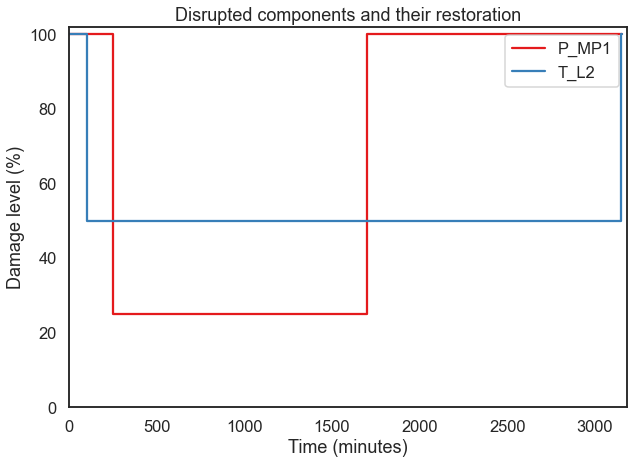
\includegraphics[width=\textwidth]{direct_effects.PNG}
		\caption{Disrupted components and their restoration}
	\end{subfigure}~
	\begin{subfigure}[h]{0.45\textwidth}
		\centering
		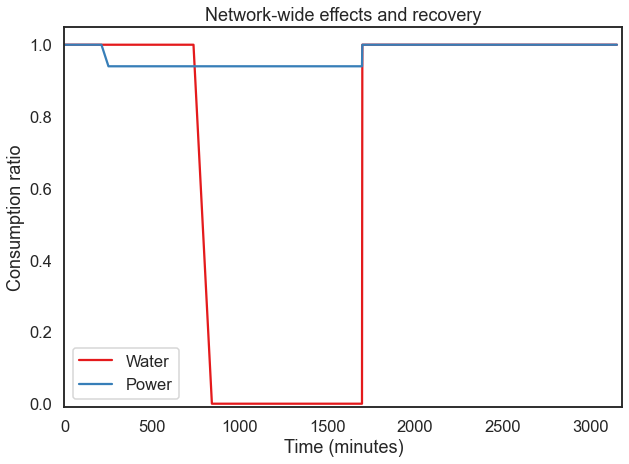
\includegraphics[width = 1.1\textwidth]{indirect_effects.PNG}
		\caption{Network-wide effects}
	\end{subfigure}
	\caption{Output plots from the integrated simulation model}
	\label{fig:graphs}
\end{figure}

\section{Save the results}
The data related to interdependent effects can be stored to local directory as follows:

\begin{sphinxVerbatim}[commandchars=\\\{\}]
location = MAIN_DIR/"dreaminsg_integrated_model/data/disruptive_scenarios/test1"
bf_simulation.write_results(time_tracker, power_consump_tracker, water_consump_tracker, location, plotting=False)
\end{sphinxVerbatim}

\chapter{Support}
The model is still in development stage. To report any issues in the model, suggest changes, or obtain support with installation or use, please write to {\href{mailto:srijith.balakrishnan@ethz.ch}{srijith.balakrishnan[at]sec.ethz.ch}}



%\renewcommand{\indexname}{Index}
%\printindex
\bibliographystyle{iitm}
\bibliography{sample}

\end{document}